\documentclass[10pt]{article}
% Shared preamble for margin-stack prototypes.
% Mirrors the production geometry: 2.6cm-wide rungs, optional 0.3cm spine at
% x=2.85-3.15, \rmfamily labels (Palatino under the real build).
\usepackage{tikz}
\usetikzlibrary{positioning,calc,patterns,decorations.pathmorphing,decorations.pathreplacing}
\usepackage{xcolor}
\usepackage[paperwidth=20cm,paperheight=25cm,margin=8mm]{geometry}
\pagestyle{empty}

% Volume accents (from books/shared/tex/theme-colors-vol*.tex)
\definecolor{crimson}{HTML}{A51C30}      % vol1  Harvard Crimson
\definecolor{ethzblue}{HTML}{1F407A}     % vol2  ETH Zurich Blue
\definecolor{amethyst}{HTML}{581C87}     % vol3  Amethyst
\definecolor{emeraldpine}{HTML}{1A4D3E}  % vol4  Emerald Pine

% One rung. #1 y-bottom  #2 height  #3 label  #4 intensity 0-100  #5 accent
\newcommand{\protorung}[5]{%
  \ifnum#4=0
    \def\fillcol{black!5}\def\textcol{black!30}%
  \else
    \def\fillcol{#5!#4!white}%
    \ifnum#4>50 \def\textcol{white}\else \def\textcol{#5}\fi
  \fi
  \node[draw=white,line width=0.5pt,fill=\fillcol,minimum width=2.6cm,
        minimum height=#2 cm,anchor=south west,inner sep=0pt] (b) at (0,#1) {};
  \node[anchor=west,text=\textcol,font=\rmfamily\scriptsize\bfseries]
        at ($(b.west)+(0.12,0)$) {#3};
}

% Rung with a right-aligned secondary label (cadence, rate, count).
% #1 y  #2 h  #3 label  #4 right-label  #5 intensity  #6 accent
\newcommand{\protorungrt}[6]{%
  \ifnum#5=0
    \def\fillcol{black!5}\def\textcol{black!30}%
  \else
    \def\fillcol{#6!#5!white}%
    \ifnum#5>50 \def\textcol{white}\else \def\textcol{#6}\fi
  \fi
  \node[draw=white,line width=0.5pt,fill=\fillcol,minimum width=2.6cm,
        minimum height=#2 cm,anchor=south west,inner sep=0pt] (b) at (0,#1) {};
  \node[anchor=west,text=\textcol,font=\rmfamily\scriptsize\bfseries]
        at ($(b.west)+(0.12,0.09)$) {#3};
  \node[anchor=west,text=\textcol,font=\rmfamily\fontsize{4.6}{5}\selectfont,opacity=0.85]
        at ($(b.west)+(0.12,-0.12)$) {#4};
}

% Vertical cross-cutting spine at x=2.85..3.15 (vol1 data bar / vol3 trajectory).
% #1 y-bottom  #2 y-top  #3 word  #4 intensity  #5 accent
\newcommand{\protospine}[5]{%
  \fill[#5!#4!white,rounded corners=1.5pt] (2.85,#1) rectangle (3.15,#2);
  \pgfmathsetmacro{\midy}{(#1+#2)/2}
  \ifnum#4>50 \def\spinecol{white}\else \def\spinecol{#5}\fi
  \node[rotate=90,text=\spinecol,font=\rmfamily\fontsize{5}{6}\selectfont\bfseries]
        at (3.0,\midy) {#3};
}

% Caption under a prototype.
\newcommand{\protocap}[2]{%
  \begin{minipage}[t]{3.0cm}\raggedright
  \textbf{\footnotesize #1}\\[1pt]{\fontsize{6.5}{8}\selectfont #2}
  \end{minipage}}

% vol3-scale rung: 4.8pt label, matching tex/agent-stack-vol3.tex exactly.
\newcommand{\protorungsm}[5]{%
  \ifnum#4=0 \def\fillcol{black!5}\def\textcol{black!30}%
  \else \def\fillcol{#5!#4!white}%
    \ifnum#4>50 \def\textcol{white}\else \def\textcol{#5}\fi \fi
  \node[draw=white,line width=0.4pt,fill=\fillcol,minimum width=2.6cm,
        minimum height=#2 cm,anchor=south west,inner sep=0pt] (b) at (0,#1) {};
  \node[anchor=west,text=\textcol,font=\rmfamily\fontsize{4.8}{5.2}\selectfont\bfseries]
        at ($(b.west)+(0.12,0)$) {#3};
}
\newcommand{\protorungsmrt}[6]{%
  \ifnum#5=0 \def\fillcol{black!5}\def\textcol{black!30}%
  \else \def\fillcol{#6!#5!white}%
    \ifnum#5>50 \def\textcol{white}\else \def\textcol{#6}\fi \fi
  \node[draw=white,line width=0.4pt,fill=\fillcol,minimum width=2.6cm,
        minimum height=#2 cm,anchor=south west,inner sep=0pt] (b) at (0,#1) {};
  \node[anchor=west,text=\textcol,font=\rmfamily\fontsize{4.8}{5.2}\selectfont\bfseries]
        at ($(b.west)+(0.12,0.07)$) {#3};
  \node[anchor=west,text=\textcol,font=\rmfamily\fontsize{3.9}{4.4}\selectfont,opacity=0.85]
        at ($(b.west)+(0.12,-0.09)$) {#4};
}

\begin{document}
\noindent{\Large\bfseries Volume IV margin stack --- five candidate forms}\\[2pt]
{\footnotesize Shown at production size (2.6\,cm rung width, the same column vol1/vol2/vol3 use).
Shading is the \emph{memory} chapter: brain tier active, body and nervous tiers as context.}\\[8mm]

% ---------- A ----------
\begin{minipage}[t]{3.15cm}
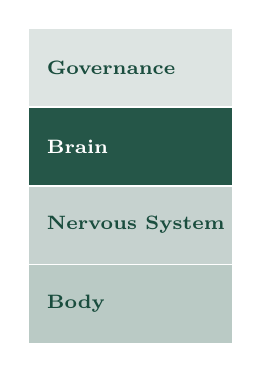
\begin{tikzpicture}
  \protorung{3.0}{1.0}{Governance}{15}{emeraldpine}
  \protorung{2.0}{1.0}{Brain}{95}{emeraldpine}
  \protorung{1.0}{1.0}{Nervous System}{25}{emeraldpine}
  \protorung{0.0}{1.0}{Body}{30}{emeraldpine}
\end{tikzpicture}\\[3mm]
\protocap{A. Organ names only}{The strictest read of vol1. Four words, nothing else. Cheapest to build, least informative.}
\end{minipage}\hfill
% ---------- B ----------
\begin{minipage}[t]{3.15cm}
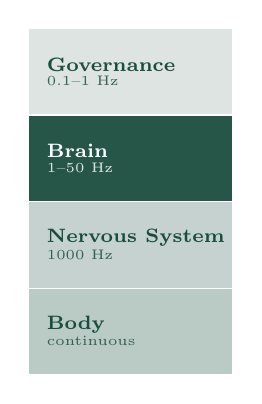
\begin{tikzpicture}
  \protorungrt{3.3}{1.1}{Governance}{0.1--1 Hz}{15}{emeraldpine}
  \protorungrt{2.2}{1.1}{Brain}{1--50 Hz}{95}{emeraldpine}
  \protorungrt{1.1}{1.1}{Nervous System}{1000 Hz}{25}{emeraldpine}
  \protorungrt{0.0}{1.1}{Body}{continuous}{30}{emeraldpine}
\end{tikzpicture}\\[3mm]
\protocap{B. + cadence}{Each tier carries the rate that defines it. Restores the density four rungs otherwise lose.}
\end{minipage}\hfill
% ---------- C ----------
\begin{minipage}[t]{3.15cm}
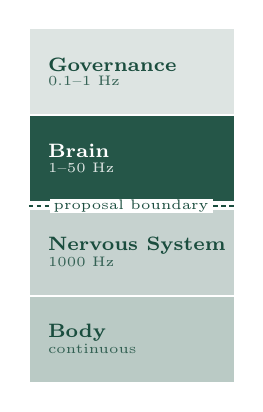
\begin{tikzpicture}
  \protorungrt{3.4}{1.1}{Governance}{0.1--1 Hz}{15}{emeraldpine}
  \protorungrt{2.3}{1.1}{Brain}{1--50 Hz}{95}{emeraldpine}
  \protorungrt{1.1}{1.1}{Nervous System}{1000 Hz}{25}{emeraldpine}
  \protorungrt{0.0}{1.1}{Body}{continuous}{30}{emeraldpine}
  \fill[white] (0,2.2) rectangle (2.6,2.3);
  \draw[emeraldpine,line width=0.8pt,dash pattern=on 1.6pt off 1.3pt]
        (0,2.25) -- (2.6,2.25);
  \node[fill=white,inner xsep=1.5pt,inner ysep=0.4pt,text=emeraldpine,
        font=\rmfamily\fontsize{4.0}{4.6}\selectfont] at (1.30,2.25) {proposal boundary};
\end{tikzpicture}\\[3mm]
\protocap{C. + privilege boundary}{Draws the one line the volume argues about: where a proposal becomes a command.}
\end{minipage}\hfill
% ---------- D ----------
\begin{minipage}[t]{3.15cm}
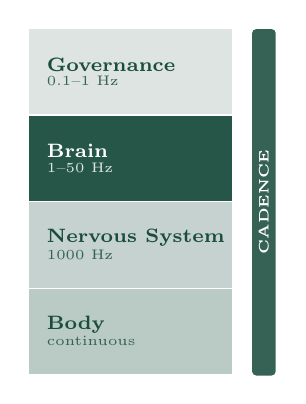
\begin{tikzpicture}
  \protorungrt{3.3}{1.1}{Governance}{0.1--1 Hz}{15}{emeraldpine}
  \protorungrt{2.2}{1.1}{Brain}{1--50 Hz}{95}{emeraldpine}
  \protorungrt{1.1}{1.1}{Nervous System}{1000 Hz}{25}{emeraldpine}
  \protorungrt{0.0}{1.1}{Body}{continuous}{30}{emeraldpine}
  \protospine{0.0}{4.4}{CADENCE}{88}{emeraldpine}
\end{tikzpicture}\\[3mm]
\protocap{D. + cadence spine}{Mirrors vol1's Data bar and vol3's TRAJECTORY spine. Names the cross-cutting quantity.}
\end{minipage}\hfill
% ---------- E ----------
\begin{minipage}[t]{3.5cm}
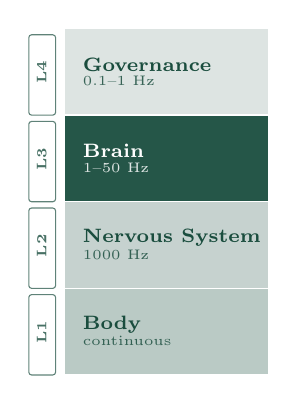
\begin{tikzpicture}
  \foreach \y/\n in {3.3/4, 2.2/3, 1.1/2, 0.0/1} {
    \node[draw=emeraldpine!70,line width=0.4pt,rounded corners=1pt,
          minimum width=0.34cm,minimum height=1.02cm,anchor=south west,inner sep=0pt]
          at (-0.45,\y) {};
    \node[rotate=90,text=emeraldpine,opacity=0.8,
          font=\rmfamily\fontsize{5}{6}\selectfont\bfseries] at (-0.28,\y+0.55) {L\n};
  }
  \protorungrt{3.3}{1.1}{Governance}{0.1--1 Hz}{15}{emeraldpine}
  \protorungrt{2.2}{1.1}{Brain}{1--50 Hz}{95}{emeraldpine}
  \protorungrt{1.1}{1.1}{Nervous System}{1000 Hz}{25}{emeraldpine}
  \protorungrt{0.0}{1.1}{Body}{continuous}{30}{emeraldpine}
\end{tikzpicture}\\[3mm]
\protocap{E. + layer gutter}{Mirrors vol2's Part boxes. Ties each tier to the layer number the prose already uses.}
\end{minipage}

\clearpage
\noindent{\large\bfseries Detail (2$\times$)}\\[4mm]
\noindent
\begin{minipage}[t]{5.4cm}\scalebox{2}{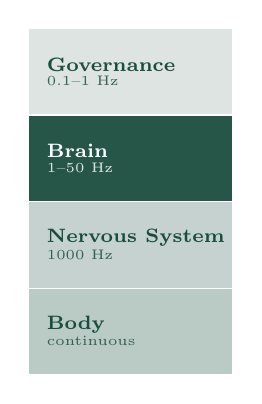
\begin{tikzpicture}
  \protorungrt{3.3}{1.1}{Governance}{0.1--1 Hz}{15}{emeraldpine}
  \protorungrt{2.2}{1.1}{Brain}{1--50 Hz}{95}{emeraldpine}
  \protorungrt{1.1}{1.1}{Nervous System}{1000 Hz}{25}{emeraldpine}
  \protorungrt{0.0}{1.1}{Body}{continuous}{30}{emeraldpine}
\end{tikzpicture}}\\[3mm]\protocap{B at 2$\times$}{Legibility check for the cadence line.}\end{minipage}\hfill
\begin{minipage}[t]{6.4cm}\scalebox{2}{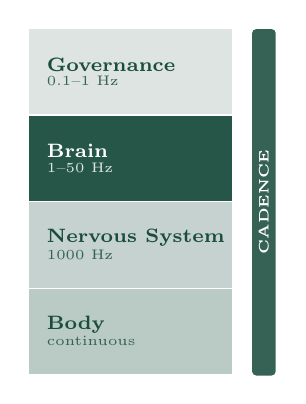
\begin{tikzpicture}
  \protorungrt{3.3}{1.1}{Governance}{0.1--1 Hz}{15}{emeraldpine}
  \protorungrt{2.2}{1.1}{Brain}{1--50 Hz}{95}{emeraldpine}
  \protorungrt{1.1}{1.1}{Nervous System}{1000 Hz}{25}{emeraldpine}
  \protorungrt{0.0}{1.1}{Body}{continuous}{30}{emeraldpine}
  \protospine{0.0}{4.4}{CADENCE}{88}{emeraldpine}
\end{tikzpicture}}\\[3mm]\protocap{D at 2$\times$}{Spine width matches vol1/vol3 exactly (0.3\,cm at x=2.85).}\end{minipage}
\end{document}
